\chapterauthor{Lars Vilhuber}{Cornell University}
\chapter{Protecting Confidential Data through Non-Statistical Methods}

This chapter will rely on and update previous overviews of how researchers, citizens, and administrators can reliably and securely access confidential data, i.e., data that cannot be simply published as ``open data''. I will discuss various legal, technical, and practical ways of securing access to data that is needed for computations. This obviously depends on the type and complexity of the computations, but also depends on the who, how, and where access is needed.

It might seem appropriate here to define what type of data I will be talking about. Several designations circulate in the various communities that create, handle, and use data: private, sensitive, confidential, proprietary. These terms are not quite interchangeable. Data may be sensitive, because they might contain attributes which could create a risk of harm to individuals or other entities described by the data. However, some sensitive data may be publicly available. In some US states, arrest records will list the name and home address of the arrested individual, but do not necessarily list if the person was ever convicted for the offense for which they were arrested. This might create harm for the individual, but the data themselves are public, and not confidential. Data might also be owned by a specific individual or institution, thus in private ownership, but not be confidential. Often, such data are referred to as proprietary. For instance, the well-known ``S\&P 500'' data are owned by a company called Standard and Poor's, can be viewed and downloaded by anybody (f.i. \cite{sp_dow_jones_indices_llc_sp_2020}), but cannot be redistributed by the downloading user: they are proprietary, but certainly not sensitive or confidential. In general, I will therefore refer to ``confidential'' data as being the key attribute that data custodians are concerned about, regardless of whether the data are proprietary or sensitive. 

I specifically exclude from this discussion mechanisms to obtain or collect confidential data from individual respondents (people and firms). Interested readers should consult \cite{groves_survey_2009}. This chapter will focus on access by analysts once data has been collected.
%, with one exception: we will describe some of the foundational aspects of multi-party computing (legal frameworks, consent issues, etc.), though all of the technical aspects of multi-party computing are left to the various chapters in Part 4.

In writing this chapter, I will rely on a variety of publications. \cite{fcsm_report_2005} touches on a few of these mechanisms, and an update is being prepared as of this writing. I have previously written about access options to firm-level data \cite{vilhuber_methods_2013}, which in turn referenced older summaries such as \cite{weinberg_access_2007}. I will use framing from \cite{desai_five_2016} and \cite{altman_towards_2015}. Astonishingly, many of the access methods in use today are not very different from those implemented nearly 20 years ago, but I will briefly describe several newer approaches, relying on previous work by myself and co-authors \cite{shen_physically_2021}.

\section{Framing: Four Regions, Five Safes}

Statistical techniques for disclosure avoidance, and secure computational methods, are conducted with the end goal of reducing the sensitivity of  data so that public statistical inferences can be made. The end goal is necessarily data that is publicly available, though that may be a statistical summary as compact as a single number, or even just a qualitative range of numbers, e.g., "positive". In some cases, data is processed in such a way that fairly high-dimensional data can be made publicly available to researchers to use as they wish. In other cases, there may be no statistical protection mechanism that simultaneously allows for detailed analysis and valid inference in the public domain, and other mechanisms must be used. It is clear that to resolve the tension between inference and accessibility of data, there is no single omnibus solution. Data custodians, statisticians, and ethicists have long recognized this. 

Conceptually, it is useful to distinguish between raw data, data transformed for disclosure avoidance purposes in such a way as to be amenable for statistical processing by the analyst, and the final statistics used for inference. Consider the transformed data first. If the reduction in sensitivity of the confidential data is such that it can be made available with negligible expected harm, while maintaining analytical validity, it can be published without restrictions. However, if despite extensive application of disclosure avoidance risks, the data could still potentially lead to negative outcomes for some respondents, a data custodian may decide to require certain safeguards or promises by analysts before they can download the data. In the extreme, if the only way to maintain the utility of the data is to retain direct identifiers in the clear, the data custodian may want to retain very tight control over who can access the data, where that access occurs, and for what purpose. 

This is the gist of a classification of tradeoffs proposed by \cite{altman_towards_2015},  a simplified depiction of which is provided in Figure~\ref{fig:altman-2015-mod}. In \cite{altman_towards_2015}, various combinations of identifiability of the transformed data and expected harm are mapped into four levels of `privacy controls'. Identifiability, which in \cite{altman_towards_2015} is tied to specific disclosure avoidance methods, ranges from the ``strongly protected'' to ``not protected at all'', whereas expected harm may range from ``negligible'' to ``catastrophic''.\footnote{See  the Harvard Data Policy  \cite{harvard_university_data_nodate} for a framing (and colorization) of these levels of sensitivity in data.}
  Level 1 corresponds to the public-use data case - no controls are imposed on the protected data. For Level 2, analysts must subject themselves, or are subject to by virtue of the legal environment, to terms of use, click-through agreements, notices, and the like. For Level 3, the data custodian requires an approval process - not only must the analyst agree to conditions, but this is tied to an approval process, possibly by some third parties (such as institutional review or ethics boards). Finally, for Level 4, much tighter controls are imposed through ``data enclaves'' (which we will define shortly). 

% https://docs.google.com/presentation/d/17AH-hcfGATG1pxZRpB-2FmF27CK2xMfjpkddZZiy5DU/edit#slide=id.p
\begin{figure}
    \centering
    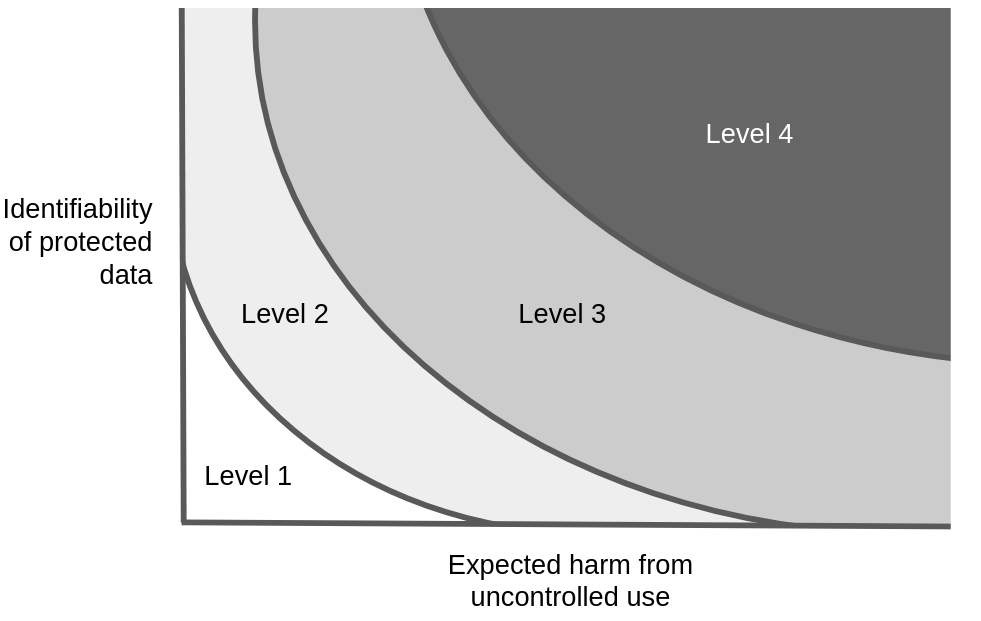
\includegraphics[width=\textwidth]{altman-2015-mod.png}
    \caption{Regions of equivalent security-access tradeoffs}
    \label{fig:altman-2015-mod}
\end{figure}

An alternative conceptualization specifically breaks out five dimensions of access control for confidential data - the transformed intermediate data mentioned earlier. It therefore focuses on the various environments associated with Levels 2-4 from Figure~\ref{fig:altman-2015-mod}. This is known as the ``Five Safes'' model \cite{desai_five_2016}, and is used by many statistical agencies and data custodians, such as the UK Government \cite{uk_government_digital_2020}, Statistics Canada \cite{statistics_canada_information_2018}, and regional governments such as Canada's province of British Columbia \cite{bc_ministry_of_citizens_services_privacy_nodate}.

The ``Five Safes'' model proposes the following ``safes'' or dimensions:  projects,  people,  settings, data, and output. \textit{Safe projects} is how the data custodian assesses the overall use of the data as proposed by an analyst. An evaluation may be required by law, as a requirement of an ethics review, or as a matter of policy.\footnote{We focus here on project vetting for the purpose of disclosure avoidance, and not for other purposes, such as congruence with policy objectives. An example of the latter might be a firm or a government agency only allowing for projects that show the data provider in a positive light.} By defining what \textit{safe people} are, the data custodian identifies who can be trusted, and what ``trusted'' means. Thus, whereas a safe project may be defined as a research project, safe people may be defined as researchers affiliated with a recognized academic institution --- excluding, for whatever reason, non-academic researchers. It may also be defined through a legal definition, such as the British Digital Economy Act's ``accredited researchers'' \cite{uk_government_digital_2020}, or by having satisfied some training requirements. 
The environment in which data access happens is described through \textit{safe settings}. This typically involves both technical and physical security of the place where access to and computing on the transformed data occurs. 

\textit{Safe data} and \textit{safe outputs} more narrowly cover what the rest of this book will address: How data are transformed, first from the highly confidential raw data to the transformed data accessed by \textit{safe people} (analysts, researchers), and subsequently, how the results from the analysis are processed to be able to release them to the general public. These two dimensions cover two distinct parts of the overall research workflow, but do not necessarily entail the use of different methods. For instance, both might use aggregation. Safe data might be created via micro-aggregation, for instance of worker-level data to the firm-level, where the firm-level data is still subject to certain access restrictions. Safe outputs might be those created by aggregating to coarse geographic granularity, and subsequently publishing without further access restrictions. 

It should be clear that these five dimensions intersect with each other to provide a specified (perceived) level of control over the disclosure risk in the underlying raw data. For instance, the choice of safe settings will influence the strength of the disclosure avoidance methods applied to create safe data. The types of projects chosen may affect the methods used for the creation of safe outputs. In almost all circumstances, the ultimate goal is to produce analytical results that are  ``safe'' to be published in broadly accessible outlets, such as academic papers, newspaper articles, or websites of statistical agencies. 

For many researchers, a key difference will lie in whether the analysis (a \textit{project}) is conducted on \textit{safe outputs}, in an open research environment, or on \textit{safe data}, in a controlled environment (\textit{safe setting}), and subject to output control (\textit{safe outputs}, again). Figure~\ref{fig:research_environments} illustrates (simplifications of) these two cases. Statisticians and computer scientists need to be aware of what particular environment is the target of a particular application of an \ac{SDL} technique. 

% Source: https://docs.google.com/presentation/d/1EWNopNdcamhDv1FYaFWIgfGdFmJLXTXQDN4O453jYIU/edit#slide=id.p

\begin{figure}
    \centering
        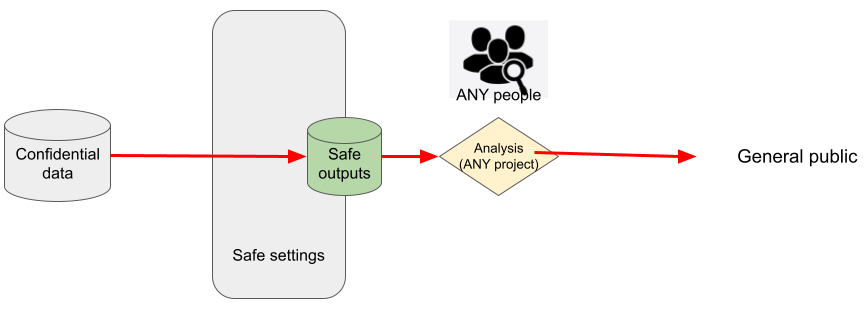
\includegraphics[width=1\textwidth]{research-environment-1.png} \\
        (a) Open research environment\\
        
        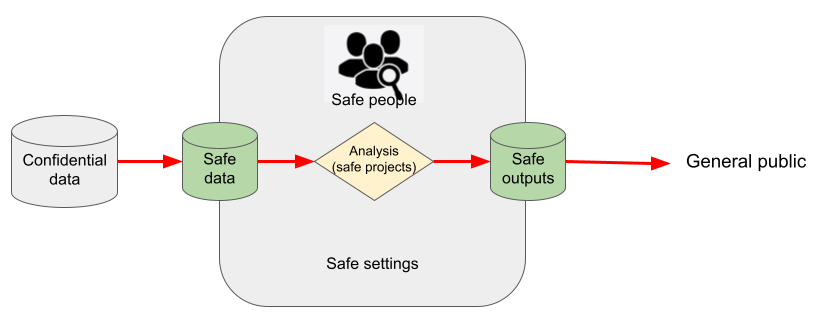
\includegraphics[width=1\textwidth]{research-environment-2.png}\\
         (b) Controlled research environment

    
    \caption{Research environments}
    \label{fig:research_environments}
\end{figure}

In what follows, I will describe in more detail the determinants of controlled resarch environments, or as I will call them, ``access mechanisms'', which are identified by different configurations of safe people, settings, and projects. 

\section{Safe People, Settings, and Projects: Access Mechanisms}

I now discuss in more detail the three dimensions --- safe people, safe settings, and safe projects --- which jointly define  various access mechanisms. Put differently, when data providers choose how to provide access to sensitive data, they pick a combination of all five dimensions, but I will treat the combination of people, settings, and projects as those defining an "access mechanism" within which safe data is made available, and which produces safe outputs through the research efforts of users. I emphasize that all five dimensions are interdependent. 

\subsection{Examples of Access Mechanisms}

To better illustrate and make concrete the three dimensions, I start by describing three examples of restricted-access mechanisms. Many more examples are discussed later in Section~\ref{sec:typical_access}, and in \cite{shen_physically_2021}.

First, consider the Norwegian ``microdata.no'' website.\footnote{{https://www.microdata.no/en/}} Researchers access confidential microdata through a website with prior registration and application process. Registered users must be affiliated with an `approved research institution' (typically but not exclusively universities) and must be holders of a Norwegian identity card. Computations are run on servers controlled by Statistics Norway, using a programming language similar to, but not identical to Stata. Outputs are protected using an automatic application of disclosure avoidance methods, and can simply be downloaded. 


Consider then the U.S. \ac{FSRDC}.\footnote{Access procedures vary by agency data, https://www.census.gov/about/adrm/ced/apply-for-access.html describes the procedures for data provided by the U.S. Census Bureau.} Researchers are authorized to access confidential microdata after application and security vetting. Minimum residency requirements apply, at least for university-based researchers. Data are processed on computers housed at the U.S. Census Bureau's computer center. Each project is independently reviewed for compliance with certain criteria. Researchers access these data from thin clients located in secure rooms located at research institutions (universities and other government agencies), access to which is controlled by the U.S. Census Bureau. A second mode of access has gained ground since the COVID pandemic, namely access for those researchers remotely from other authorized locations, such as home offices, using virtual desktop software.\footnote{Virtual or remote desktop software displays a remote computer desktop on the screen of a local computer. In some cases, interactions of the remote desktop with the local computer are inhibited, and only keyboard and mouse control are sent to the remote desktop, practically acting as if it were a thin client.  A thin client is a dedicated device used for connecting to a remote (typically virtual) desktop.} In both cases, researchers lack the ability to upload or download any materials from the remote computing facility. 

Finally, consider the \ac{NCES} restricted data licenses.\footnote{https://nces.ed.gov/statprog/rudman/j.asp, accessed 2022-04-16.} Researchers' (US-based) organization sign a licensing agreement with the agency, and submit a security plan. They must also justify the need for access to the confidential data, but need not do so on a per-project basis. Organizations are limited to research institutions, government agencies, and consulting frims. The organization-controlled standalone, secure desktop computer must be located in a separate room (controlled by the university, not the agency). Researchers can upload and download files, but commit to not downloading any of the data. 

In contrast to these access mechanisms stands the `open data' approach, typically referred to as `public use data': free and unencumbered download of data. Note that such public use data is just a limiting case of the various dimensions we will outline here, corresponding to a situation where `safe people', `safe settings', and `safe projects' are all set to infinity, obviating the need for `safe data', and putting all weight on protecting respondents on the techniques to create `safe outputs'. 

\subsection{Safe People: Exclusions, Inclusions, and Training}

Who can be trusted to handle data of varying degrees of sensitivity is one of the key aspects of any access mechanism. The open-access movement of the last decades has made access to non-sensitive data much easier in many countries, building on earlier efforts such as the Canadian `Data Liberation Initiative' \cite{currie2015social}, and leading to the widespread adoption of open data licenses \cite{statistics_canada_statistics_2012,uk_government_open_2014}. In the United States, of course, public-use micro data have been around for much longer, but as with Canada and the UK, the original files of what are now called public-use microdata samples (PUMS) were sold, not made freely available, and required users to have access to mainframes (U.S. Census Bureau, cited in \cite{anderson_american_2015}). De facto, only 85 research institutions purchased the files for the 1960 Decennial Census \cite{anderson_american_2015}. Thus, even though anybody could purchase them, there were technical requirements that prevented many from accessing these files. Today,  users can simply download the same 1960 PUMS files from IPUMS \cite{ruggles_steven_ipums_2021} onto a relatively cheap personal computer.

The 1960 PUMS files were subject to relatively simple disclosure avoidance techniques (sampling, coarsening, and de-identification), and whether the limitations on its user base due to the technical requirements were taken into account by the data curators when choosing the disclosure avoidance techniques is unknown. But today, PUMS files are available to any user, without restriction. Whether users are considered `safe' or not does not matter. 

For more sensitive files, however, many data providers restrict the user base in various ways, treating some users as ``more trusted'' then others. Such conditions may be by affiliation (university-affiliated), presumably associating users employed  by certain institutions as being more likely to be `safe'. Conditions can emphasize citizenship or residency requirements. In the Norwegian case, researchers must be affiliated with a limited list of institutions, and must have been a Norwegian resident sometime in the past. For the FSRDC, a three-year minimum residency requirement applies. Such conditions are in practice exclusionary against certain groups. Citizen science becomes nearly impossible to perform, and even journalists may have difficulty in complying with such rules, even though neither may be explicitly excluded. 

People may also be considered `safe' if they have received security and sensitivity training, though the exact type and extent of training can vary substantially across data providers and access networks. Users of the FSRDC and licensees of NCES data are required to participate yearly in IT security and confidentiality training. Users of the Norwegian data do not appear to have required training, but their host institutions may require their own training. The IDAN Network lists a comparison of user training for six different European access networks \cite{idan_network_idan_nodate}, noting that duration, requirement for presence, and frequency all vary even when the various networks are actively collaborating with each other. 

Thus, as the sensitivity of the files increases, data providers may move away from giving any user access to the data. As one dimension is relaxed (how safe the data are made to be), another dimension is tightened (who can access the data), illustrating the tradeoffs that data providers make. 

\subsection{Safe Settings and Projects: Legal and Contractual Mechanisms}

The users accessing the data do so within certain legal and contractual mechanisms: the legal component of `safe settings'. These include general laws such as the European Union's General Data Protection Regulation (GDPR) \cite{noauthor_general_2016}, or the U.S. E-government Act of 2002 \cite{noauthor_e-government_2002}, and more specific laws, such as Title 13, U.S.C., which applies specifically to data collected by the U.S. Census Bureau \cite{noauthor_title_nodate,us_census_bureau_federal_2021}. Such legal frameworks provide for monetary penalties and potential prison sentences for illegitimate uses of the data, and may define what legitimate uses are. Users of FSRDC and NCES data are both subject to such legal enforcement.

Other data providers rely not just on legal mechanisms, but may also leverage contract law for penalties, in particular when data providers and users reside in different jurisdictions. Simply put, by signing the data use agreement --- a legally enforceable contract between two parties --- users \textit{voluntarily}  commit to paying a penalty if security provisions are breached. Private or commercial providers of confidential data may rely exclusively on such mechanisms. 

Physical settings matter, and I discuss these in more detail in the next section, but even beyond the fact that some researchers must go into a \textit{locked room} on a university campus, it may matter that those researchers are \textit{on campus}, and not elsewhere. Many data access mechanisms require that users be in a specific location, even when technically it may be possible to access the remote data access mechanism from other locations. This is true for both NCES and FSRDC. I speculate that this  may affect the particular mindset of the researcher, by possibly being surrounded by other researchers working on similarly sensitive data, magnifying the effect of previously received training. 

The selection of projects also interacts in subtle ways with the legal framework and other dimensions of the Five Safes framework. In some cases, legal frameworks require that only certain types of projects be authorized. For instance, certain U.S. states allow access to their data only if the research directly improves program compliance. Often, the expected type of project serves as a filter for the type of expected output. Academic projects often result in very compact model estimates, not vast tables, and thus facilitate the type of output control (`safe outputs') where traditional disclosure avoidance methods can be manually applied. For instance, FSRDC projects that involve Census Bureau data must satisfy a limited set of criteria, and must provide a benefit towards the Census Bureau's statutory goals. Even more stringent criteria apply when the data requested are sourced from the \ac{IRS}.

Project selection can introduce subtle biases as well. While in all three example mechanisms, project selection is based on objective legal criteria, and is unlikely to bias research questions or findings, project selection when the data provider is a commercial entity may do so. Many commercial data providers may require vetting of the findings by their legal department, potentially suppressing findings that do not suit the corporate goals. 

%Talk about laws regarding illegal disclosures (exclude laws regarding illegal data collection), and contractual mechanisms (DUA, MOU, NDA) that are used in practice. Social mechanism will collapse the "Safe People" and "Safe Projects" category, also focusing on the institutional aspects of "safe people". Touch on exclusionary aspects of "safe people" - should non-academics have access, for instance, journalists? Mention open data laws (government) and open data mandates with funders. Also talk about how enforcement can play a key role - residency or citizenship as one criterion.

% for methods centered on surveys, and \cite{meyer_practical_2018} on the limits to ethical data sharing

\subsection{Safe Settings: Physical Mechanisms}

When considering the `safe settings' part of the Five Safes, physical environments play an important role, in addition to the legal setting. Physical environments in the broadest sense are those places where data is stored and processed, and where researchers sit when accessing the data. The two places are not necessarily the same, even though inevitably the place where researchers sit also has computers. Generally, one should consider the entire data access mechanism as part of the `safe settings'.

In \cite{shen_physically_2021}, we defined five aspects of data access mechanisms, by which we classified data access mechanisms currently in use, or being planned. These aspects are:
\begin{itemize}
    \item the level of \textbf{researcher agency over analysis computers} --- how much can a researcher, as opposed to an IT specialist or data custodian, manipulate the computing environment;
    \item the \textbf{location of analysis computers} --- the computers on which computations are run, whether they are located in the same space as the researcher, the data provider, or a third party;
    \item the \textbf{location of access computers} --- which historically was the same as the analysis computer, but in modern systems is generally separate;
    \item the \textbf{level of access security} over both the physical environments (rooms) and access computers;
    \item the \textbf{range of analysis methods available}.
\end{itemize}

I will briefly summarize here what each of these aspects implies for the access mechanism, and how they allow to characterize some of the most common access mechanisms; the reader is referred to \cite{shen_physically_2021} for more details. I will also point out the implications for the need for safe data, as well how access mechanisms interact with the feasibility of certain safe output mechanisms.


\subsubsection{Researcher Agency over Analysis Computers}

How much control do researcher have over the analysis computers? In some cases, researchers will have very little influence about most characteristics of the analysis computers, because these computers are managed and controlled by the data custodian, with little to no ability to change the setup. In other cases, researchers may be able to choose or request software, or define specific hardware setups. In the highest researcher agency setting, researchers have full control over the analysis computers, because it may simply be the research workstation or laptop that they use for many other activities as well. Note that this also affects how researchers can interact with those analysis computers --- is it possible to upload researcher-created scripts directly to the analysis computers, or are such insertions of computer code into the analysis computer mediated by semi-automated or manual mechanisms. 

Consider the three mechanisms outlined earlier. In the Norwegian case, users have no control over the choice of software or hardware capabilities of the analysis computers - they have low agency. In the FSRDC case, they also have no control over analysis computers, but a broad spectrum of software options are available to choose from, and others can be requested. Even when the analysis computers are accessed from home offices, this does not change: the same analysis computers are being accessed as would have been accessed from the secure on-campus room. They have medium agency over the analysis computers. Finally, in the NCES case, researchers have full agency over the analysis computers, except for certain security requirements. Any software can be loaded on the analysis computer, and scripts can be easily uploaded.

\subsubsection{Location of Analysis Computers and Data}

But where can those analysis computers be located? In many situations, the analysis computers may be located with the data \textit{provider}. This is often the case when private companies, or non-statistical government agencies, provide access to confidential data ``on premise''. In other cases, the data may be hosted with a secure and trusted third-party, a data \textit{custodian} or intermediary. For most practical purposes, these two cases are indistinguishable for the researcher --- they are primarily distinguished from the case where the analysis computer is located with the researcher. In more recent years, many data providers have moved to ``offload'' data access to a trusted third-party, although that entity often resides within the same larger organization. 

Consider again the three examples above. In both the Norwegian and the FSRDC case, analysis computers and data are located with the data provider. However, while the U.S. Census Bureau used to be its own data access provider, it has increasingly expanded use of the \acp{FSRDC} to also host data from other agencies. For those data, the U.S. Census Bureau, providing the FSRDC services, acts as a trusted third-party to other agencies of the U.S. government, such as the Bureau of Labor Statistics.%
\footnote{Another example is the French \ac{CASD}, which started as the data access portal for the French statistical agency --- \ac{INSEE} --- but has since been spun out into a public-private partnership, providing data access services to data from many French government agencies \cite{SILBERMAN_2021}.} In the NCES case, the analysis computer and the data are located in premises controlled by the researcher (or the researcher's home institution).

\subsubsection{Location of Access Computers}

Researchers may traditionally think of their ``workstation'' or ``laptop'' as the access computer, when the data are on storage media directly attached. This, in fact, is the likely modus operandi when using most public-use data. However, when processing confidential data,  the analysis computer may not be physically accessible to the researcher, and must receive instructions via a separate access computer. Naturally, the researcher must always be able to directly access the access computer, but the location ---  with the non-researcher data custodian, a third-party access provider, or with the researcher --- plays an important role. 

The NCES licensing case still leverages the traditional model of the workstation-as-the-access-computer --- access computer and analysis computer are coincident, and in researcher-controlled space. In the case of the FSRDC, the access computer is either a thin client, located in the on-campus secure room, or special software running on a researcher's laptop, from a single authorized location that is typically the researcher's home office. In the Norwegian case, a simple web browser, accessed from any computer anywhere in the world, provides access to the analysis computers. 

\subsubsection{Security of Access Computers}

Regardless of location, there is substantial variation in the implemented security of the access computers and the premises where it is located.  Data providers often require the right to approve the security arrangements, conduct audits, or otherwise directly verify that the operator is in compliance with the mandated security requirements. They may require specific third-party operators of facilities or computers. Heuristically, the security of access computers and their rooms can range from highly secure to unsecured (beyond basic computer security).

Consider the Norwegian case. Since access is web-based, even the unsecured hotel lobby computer might conceivably be used to access the system. In contrast, the physical facilities traditionally used by the FSRDC system have building requirements (specifying wall construction, window placement, alarm systems, etc.) and computer restrictions (thin clients with no local storage). While newer remote-access permissions relax some of those restrictions, they still specify locality (home locations, but not the next internet café) and software (only specific virtual desktop software will allow for access, and prevents all interaction with the host computer). In the NCES case, secure rooms are also required, with certain, lighter, requirements -- a lock on the door and restricted access appears to be sufficient \cite{national_center_for_education_statistics_appendix_nodate}. Certain security requirements are enumerated for the access computer, but they are likely to be satisfied by any regular university-managed computer.

\subsubsection{Range of Analysis Methods Available}

While somewhat overlapping with the \textbf{Researcher Agency over Analysis Computers}, we considered this to be a distinct aspect, because even when agency is low, there may well be significant differences in the available analysis methods, and these materially affect the researcher's ability to apply and incorporate disclosure avoidance methods, such as those outlined in the other chapters. 

Consider the distinction between the Norwegian system and the FSRDC. In both, researchers have no control over the analysis computer, but in the Norwegian case, there is only one possible programming language, whereas in the FSRDC case, there are many (and because agency is slightly higher, additional ones can be requested). Often, remote submission systems (similar to the Norwegian system) are limited to a single programming language, often with explicitly limited capabilities. 

\section{Typical Access Mechanisms}
\label{sec:typical_access}

There are a variety of different access mechanisms that researchers typically encounter. I already introduced three of them earlier: ``microdata.no'', FSRDC, and NCES.  I briefly sketch a few more here, see \cite{shen_physically_2021} for details. 

The simplest restricted-data access mechanism I already outlined for the NCES case: users sign an agreement, obtain the data, and work on a computer they provide, possibly in a locked room. Such a mechanism provides \textit{high agency} over the analysis computer, a simple IT setup, and allows for a \textit{wide range of analysis methods}. It is, however, potentially complex to manage at scale, when thousands such agreements are to be monitored. It is quite frequently used for surveys (PSID or HRS confidential data) or  proprietary data (Kilts Center). 

Pure licensing agreements are seldomly used nowadays for access to sensitive data provided by national statistical agencies. Those have tended to use designated physical infrastructure --- commonly called a ``\textbf{research data center}'' --- and historically physical shipment of data to analysis computers located within those spaces \cite{currie2015social}  --- therefore also known as a ``physical data enclave''. Such a system provides less researcher control over the physical location, and generally less agency over the analysis computers. Yet it also often generates diversity within such a network of research data centers, for instance in computational capacity. More and more data providers have shifted to, or even started out with a variant that incorporates a strong remote component, which may be called ``virtual data enclave'', ``virtual desktop infrastructure (VDI)'', or ``thin client''. The access computers may still be in dedicated secure rooms (the traditional model used in the FSRDC, in the Canadian RDC network, or for the German \ac{IAB}), in researcher offices (the French \acf{CASD}), or through dedicated software from researchers' homes (the newer FSRDC model) or offices. Some providers of proprietary data will also provide ``secure laptops'' that de facto use remote connection protocols to connect to corporate infrastructure. The virtual model does not necessarily modify researcher control over locations --- in all of the mentioned examples, the data custodian specifies a specific location --- but unifies the type of data and software available to hundreds or thousands of researchers. It also increases the sense of security on the data provider side, since access to the data can be terminated quickly and completely, in contrast to the other two mechanisms. Whether that constitutes a de facto increase in actual security is unknown, and may be unknowable. 

Finally, the Norwegian mechanisms, as well as the Canadian RTRA \cite{statistics_canada_real_2021} or the Australian TableBuilder, are examples of \textbf{remote submission} systems, where code is sent to a remote system through a non-interactive mechanism, and researchers then receive results once computations are completed. Computer scientists might recognize this as a variant on application programming interfaces (APIs), used for instance for geocoding of addresses, but typically with less sophisticated submission systems. Both the Canadian and Australian systems are focused primarily on custom tables, rather than more sophisticated analyses.

%\section{Organizational Mechanisms}

%Researchers do not usually negotiate over the various dimensions of the Five Safes separately or on a case-by-case basis. For medium to large organizations, including national statistical agencies, combinations of these are packages into various access mechanisms. 



\section{Discussion}

%TODO

%Increase the level of protection applied to `safe outputs', reducing the emphasis on all other dimensions, and "public-use data" is the result, as we originally pointed out. Shift some protection onto the creation of  `safe data', for instance by creating non-DP synthetic data, and relatively liberal distribution policies might be feasible, relying only on click-through user agreements, but with the downside that inference is uncertain. In other instances, such as Statistics Canada's Real Time Remote Access, the range of analysis methods as well as the set of `safe people' using it are restricted,  but inference validity is maintained and the convenience of the access is increased. Alternatively, by offering ``factually anonymous datasets'', restricting users to academic researchers at universities may be sufficient, as in the case of the German Institute for Employment Research \cite{forschungsdatenzentrum_der_ba_im_iab_scientific_nodate}.

In reading the other chapters of this book, readers may want to keep in mind that all levers of protection --- the Five Safes --- contribute to the overall protection of confidential data. In many cases,   multiple access channels will exist simultaneously, with different combinations of the level of each of the elements, which allow to analyze and derive inferences from the underlying confidential data. For instance,  the \ac{IAB} offers campus data (synthetic data that is not inference-robust), scientific use files (factually anonymized, coarsened, and with a limited number of variables), and files in the research data center of the IAB, all of which have been derived from the confidential internal data of the agency. For each decennial census, the U.S. Census Bureau provides uncontrolled public access to some tabular data without any \ac{SDL}, as mandated by law, and to other tabular data with some \ac{SDL} applied. The Bureau also provides access to public-use microdata with substantial \ac{SDL} applied, and access to lightly protected ``safe'' microdata in the \ac{FSRDC}, with substantial restrictions on ``safe projects'' and ``safe people''. The actually collected confidential microdata is distinct even from the ``safe'' data in the FSRDC, and is accessed by only a few internal researchers --- until 72 years later, as mandated by law, all microdata is made publicly available. The \ac{SDL} applied to the data in each of the three different IAB and the four different Census Bureau access mechanisms is (at least in theory) optimized for the settings, projects, and people able to conduct research through each of these access mechanisms. Clearly, there are projects (analyses) that are not feasible through some access mechanisms. For instance, it would not be reasonable to conduct analyses into the top 1\% of the earnings distribution using Census Bureau public-use microdata, because top-coding and other \ac{SDL} may severely bias or hamper such an analysis. But it is also likely not to be feasible to do custom tabulations of the ``safe'' decennial data, as such projects may not be approved or because the methods used to create ``safe outputs'' from such custom tabulations are inadequate. Borrowing a term from Meng  \cite{meng-congenial}, the \ac{SDL} both before and after the point of analysis needs to be congenial with the analysis method itself.

This would seem to be particularly true when using synthetic data, of either the classical or DP variant, as such data may be valid for some use cases, and yet not valid for others. \cite{barrientos_providing_2018}  proposed a mechanism that would signal when inferences might be invalid, though they did not offer an alternate mechanism. \cite{dwork_fienberg_2018} illustrated this in the context of interactive usage, restricting access to a subset. The idea could be expanded to a variety of protection mechanisms. In particular, suppose that users have access to a DP-synthetic public-use dataset akin to \cite{barrientos_providing_2018}. Using a \textbf{remote submission system}, researchers obtain either an inference-valid result, or a signal that the inference may not be valid. In the latter case,  researchers may be granted access to a lightly restricted ``synthetic data server'' \cite{vilhuber_usage_2016} prior to submitting to a  different remote submission system, with access to the same data as \cite{dwork_fienberg_2018}. Results from computing on the ``safe non-synthetic data'' are made into `safe outputs' using a different but also DP mechanism. Such a mechanism does not yet exist (though see \cite{vilhuber_usage_2016}), but is a logical consequence of connecting various combinations of the Five Safes in a way that reduces both human and computational burden.

%A short introduction before the first section.

%\section{Section 1}
%Please edit mychapter.tex. Here are examples of fancy options. More information can be found in README.pdf
%\subsection{a subsection}


%\begin{VF}
%``You can add a fancy quote using the VF environment''
%
%\VA{Anonymous}{Chief Scientist of Unknown Affiliation}
%\end{VF}

%\begin{shadebox}
%OMG! A shaded Box!
%\end{shadebox}

%\begin{shortbox}
%\Boxhead{Another way to do boxes}
%Think outside the box
%\end{shortbox}


%\begin{table}[b!]%2
%\tabletitle[Short Table Caption]{Long caption goes here}%}{%
%\begin{tabular}{lccc}
%\tch{Col 1}    &\tch{Col 2} &\tch{Col 3} &\tch{COl 4}\\
%\multicolumn{4}{@{}l@{}}{\tsh{Table Head}}\\[3pt]\hline\\[-6pt]
%Item 1 &19, 221 &4, 598   &3, 200\\
%Item 2 &46, 281 &6, 898 &5, 400\\
%Item 3   &27, 290 &2, 968 &3, 405\\
%Item 4    &14, 796 &9, 188 &3, 209\\
%\end{tabular}
%\end{table}
